\documentclass{article}
\usepackage{fancyvrb}
\usepackage{xcolor}
\usepackage{pygments}

\usepackage{polytexnic}
\begin{document}

\title{The Tau Manifesto}
\author{Michael Hartl}
\date{June 28, 2010}
\maketitle

\section{The circle constant} % (fold)
\label{sec:the_circle_constant}

Welcome to the \emph{Tau Manifesto}. This manifesto is dedicated to one of the most important numbers in mathematics, perhaps \emph{the} most important: the \emph{circle constant} relating the circumference of a circle to its linear dimension. For millennia, the circle has been considered the most perfect of shapes, and the circle constant captures the geometry of the circle in a single number. Surely, defining this constant properly is a task that the great mathematicians of history should---nay, \emph{must}---have gotten right\ldots

Only they didn't. The traditional choice of circle constant, of course, is $\pi$---but, as mathematician \href{http://www.math.utah.edu/~palais/}{Bob Palais} notes in his delightful article ``$\pi$ Is Wrong!'',\footnote{Palais, Robert. ``$\pi$ Is Wrong!'', \emph{The Mathematical Intelligencer}, Volume~23, Number~3, 2001, pp.~7--8. (``$\pi$ Is Wrong!'' is available online at \href{http://www.math.utah.edu/~palais/pi.html}{Bob Palais' pi page}.)} $\pi$ \emph{is wrong}. The traditional definition for the circle constant sets $\pi$ (pi) equal to the ratio of the circle's circumference to its diameter:\footnote{The symbol $\equiv$ means ``is defined as''.}


\[
  \pi \equiv \frac{C}{D} = 3.14159265\ldots
\]

\noindent Unfortunately, this definition is off by a factor of two in the denominator. Since a circle is the set of points a fixed distance---the \emph{radius}---from a given point, the most natural definition for the circle constant uses $r$ in place of $D$:

\[
  \mathrm{circle\ constant} = \frac{C}{r}
\]

Although he argues persuasively in favor of the above definition, even the plucky Professor Palais can't quite bring himself to take his idea seriously. Indeed, his initial inclination is to \emph{redefine} $\pi$ as

\[
  \pi \equiv \frac{C}{r}
\]

\noindent Given how deeply entrenched $\pi$ is in its current form, this redefinition is a complete nonstarter; it suggests, with a wistful tone, a ``\emph{wouldn't it have been nice if\ldots}'' sentiment that has no chance of any real-world usage---thereby \emph{approaching} the truth but stopping short when the implications become too uncomfortable.\footnote{George Orwell called this phenomenon \href{http://en.wikipedia.org/wiki/Crimestop}{\emph{crimestop}}.} Of course, using $\pi$ in the manner above would be hopelessly confusing, so ultimately Dr. Palais does introduce a separate symbol for the circle constant, which he calls ``one turn''.  As we'll see, the description is prescient, but the symbol, lamentably, is absurd (\hyperref[fig:palais-tau]{Figure~}\ref{fig:palais-tau}).\footnote{Why propose an absurd symbol that has no chance of ever being used in a serious context? As I said: \href{http://en.wikipedia.org/wiki/Crimestop}{\emph{crimestop}}.}


\begin{figure}
\begin{center}

\includegraphics{images/figures/palais-tau.png}
\end{center}
\caption{The absurd symbol used for the circle constant in ``$\pi$ Is Wrong!''.\label{fig:palais-tau}}
\end{figure}

The \emph{Tau Manifesto} is dedicated to the proposition that the proper response to ``$\pi$ is wrong'' is ``No, \emph{really}.'' Moreover, the true circle constant deserves a proper name. The \emph{Tau Manifesto} proposes that this name---as I hope you will not be surprised to learn---should be the Greek letter $\tau$ (tau):

\[
  \tau \equiv \frac{C}{r} = 6.2831853071796586\ldots
\]

\noindent This symbol is neither confusing nor absurd. The rest of this manifesto is will show that the \emph{number} $\tau$ is the correct choice, and will show through usage (\hyperref[sec:the_number_tau]{Section~}\ref{sec:the_number_tau}) and direct argumentation (\hyperref[sec:why_tau]{Section~}\ref{sec:why_tau}) that the \emph{letter} $\tau$ is a natural choice as well.

 \subsection{A powerful enemy} % (fold)

Before proceeding with the demonstration that the number $\tau$ is the natural choice for the circle constant, let us first acknowledge what we are up against---for there is a powerful conspiracy, centuries old, determined to propagate pro-$\pi$ propaganda. Entire \href{http://www.amazon.com/exec/obidos/ISBN=0802713327/parallaxproductiA/}{books} \href{http://www.amazon.com/Pi-Sky-Counting-Thinking-Being/dp/0198539568}{are} \href{http://www.amazon.com/exec/obidos/ISBN=0312381859/parallaxproductiA/}{written} extolling the virtues of $\pi$. I mean, \href{http://www.amazon.com/exec/obidos/ISBN=0387989463/parallaxproductiA/}{\emph{books}}\emph{!} And $\pi$ perfidy has captured even the highest levels of geekdom; for example, for the 2010 ``$\pi$ Day'' celebration (taking place annually on March~14), \href{http://www.google.com/}{Google} \emph{changed its logo} to honor $\pi$  (\hyperref[fig:google-pi-day]{Figure~}\ref{fig:google-pi-day}).  Meanwhile, some people memorize dozens, hundreds, even \emph{thousands} of digits of this mystical number. What kind of sad sack memorizes dozens of digits of $\pi$ (\hyperref[fig:michael_hartl]{Figure~}\ref{fig:michael_hartl})?

\begin{figure}
\begin{center}
\image{images/figures/google-pi-day.gif}
\end{center}
\caption{The Google logo on March 14, 2010.\label{fig:google-pi-day}}
\end{figure}

\begin{figure}
\begin{center}
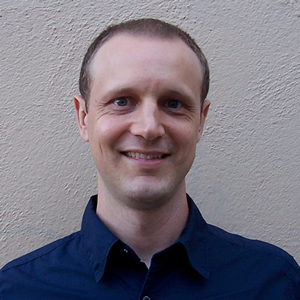
\includegraphics{images/figures/michael_hartl.jpg}
\end{center}
\caption{This poor bastard once memorized $\pi$ to 50 decimal places.\label{fig:michael_hartl}}
\end{figure}

Truly, defenders of $\tau$ face a mighty opponent. And yet, we have a powerful ally---for the truth is on our side.

% section the_most_important_number (end)

\section{The number tau} % (fold)
\label{sec:the_number_tau}

If you look through the equations of mathematics, you will find that the combination $2\pi$ occurs (if you are a $\pi$-partisan) with alarming frequency. For example, consider integrals over all angles in polar coordinates:

\[
  \int_0^{2\pi}\int_0^r f(r, \theta)\, dr d\theta
\]

\noindent The same factor of $2\pi$ occurs in the definition of the \href{http://en.wikipedia.org/wiki/Normal_distribution}{normal distribution}:

\[
  \frac{1}{\sqrt{2\pi}\sigma}e^{-\frac{(x-\mu)^2}{2\sigma^2}}
\]

\noindent It recurs in \href{http://en.wikipedia.org/wiki/Cauchy's_integral_formula}{Cauchy's integral formula}:

\[
  f(a) = \frac{1}{2\pi i}\int\frac{f(z)}{z-a}\,dz
\]

\noindent ``$\pi$ Is Wrong'' contains many more examples, and the lesson is clear: there's something suspicious about $\pi$, and something natural about $2\pi$. To get to the bottom of the mystery, we must consider the nature of the circle, and especially the nature of \emph{angle}.

  \subsection{The nature of angle} % (fold)
  \label{sec:the_nature_of_angle}

There is an intimate relationship between circles and \emph{angles}, as shown in \hyperref[fig:angle-arclength]{Figure~}\ref{fig:angle-arclength}. Although the lines in the figure cut off different lengths of arc (i.e., different \emph{arclengths}) from two concentric circles with different radii, the angle~$\theta$ is the same in each case. The problem of angle measurement is to create a system that captures this arclength- and radius-invariance.

\begin{figure}
\begin{center}
\image{images/figures/angle-arclength.png}
\end{center}
\caption{An angle $\theta$ with two concentric circles.\label{fig:angle-arclength}}
\end{figure}

Perhaps the most elementary angle system is \emph{degrees}, which arbitrarily breaks a circle into 360 equal parts. One result of this system is the set of special angles familiar to students of trigonometry (\hyperref[fig:degree-angles]{Figure~}\ref{fig:degree-angles}). 

\begin{figure}
\begin{center}
\image{images/figures/degree-angles.png}
\end{center}
\caption{Some important angles, in degrees.\label{fig:degree-angles}}
\end{figure}

A more fundamental system of angle measure involves a direct comparison of the arclength $s$ with the radius $r$. Although the arclengths in \hyperref[fig:angle-arclength]{Figure~}\ref{fig:angle-arclength} differ, the lengths grow proportional to the radius, so that the \emph{ratio} of the arclength to the radius is the same for each:

\[
s\propto r \Rightarrow \frac{s_1}{r_1} = \frac{s_2}{r_2}
\]

\noindent This suggests the following definition of \emph{radian angle measure}:

\[ \theta = \frac{s}{r} \]

\noindent This definition has the required properties of arclength- and radius-independence, and it leads to elegant formulas throughout mathematics. For example, the formula for the derivative of $\sin\theta$ is true only when $\theta$ is in radians:

\[
  \frac{d}{d\theta}\sin\theta = \cos\theta \mathrm{\ \ \ \ (only\ when\ } \theta\mathrm{\ is\ in\ radians)}
\]

Naturally, the special angles in \hyperref[fig:degree-angles]{Figure~}\ref{fig:degree-angles} can be expressed in radians, and when you took high-school trigonometry you probably memorized the special values shown in \hyperref[fig:pi-angles]{Figure~}\ref{fig:pi-angles}. (I call this system of measure $\pi$-radians to emphasize that they are written in terms of $\pi$.)

\begin{figure}
\begin{center}
\image{images/figures/pi-angles.png}
\end{center}
\caption{Some important angles, in $\pi$-radians.\label{fig:pi-angles}}
\end{figure}

\noindent We now begin to see just how ridiculous $\pi$ is, for a moment's reflection shows that the so-called ``special'' angles are simply  \emph{rational fractions} of a full circle, as shown in \hyperref[fig:angle-fractions]{Figure~}\ref{fig:angle-fractions}.

\begin{figure}
\begin{center}
\image{images/figures/angle-fractions.png}
\end{center}
\caption{The ``important'' angles are rational fractions of a full circle.\label{fig:angle-fractions}}
\end{figure}

\noindent We can now revisit the definition of radian angle measure, writing the arclength in terms of the fraction of the full circumference:

\[ \theta = \frac{s}{r} = \frac{fC}{r} =  f\left(\frac{C}{r}\right) \equiv f\tau \]

\noindent Notice how naturally $\tau$ falls out of this analysis. If you are a believer in $\pi$, the resulting diagram of angles---shown in \hyperref[fig:tau-angles]{Figure~}\ref{fig:tau-angles}---will shake your faith to its core. Although there are other arguments in $\tau$'s favor, \hyperref[fig:tau-angles]{Figure~}\ref{fig:tau-angles} may be the most striking. Indeed, upon comparing \hyperref[fig:tau-angles]{Figure~}\ref{fig:tau-angles} with \hyperref[fig:angle-fractions]{Figure~}\ref{fig:angle-fractions}, I consider it decisive.

\begin{figure}
\begin{center}
\image{images/figures/tau-angles.png}
\end{center}
\caption{Some important angles, in radians.\label{fig:tau-angles}}
\end{figure}

We see from \hyperref[fig:tau-angles]{Figure~}\ref{fig:tau-angles} the genius of Bob Palais' description of ``one turn'' for the circle constant: $\tau$ is the radian angle measure for one \emph{turn} of a circle. Moreover, note that with $\tau$ there is \emph{nothing to memorize}; the radian angle measure for an eighth of a circle---one slice of pizza---is simply $\tau$/8. We also see from \hyperref[fig:pi-angles]{Figure~}\ref{fig:pi-angles} where those pesky factors of $2\pi$ come from: one turn of a circle is $2\pi$. These unnecessary factors of $2$ are annoying in themselves, but far more serious is their tendency to \emph{disappear} when divided by any even number. The absurd results, such as $\pi$/2 for a \emph{quarter} circle, obscure the underlying relationship between angular measure and the circle constant.

To those who maintain that it ``doesn't matter'' whether we use $\pi$ or $\tau$ when teaching trigonometry, I simply ask you to view \hyperref[fig:pi-angles]{Figure~}\ref{fig:pi-angles}, \hyperref[fig:angle-fractions]{Figure~}\ref{fig:angle-fractions}, and \hyperref[fig:tau-angles]{Figure~}\ref{fig:tau-angles} through the eyes of a child. You will see that, from the perspective of a beginner, \emph{using $\pi$ instead of $\tau$ is a pedagogical disaster.}

  \subsection{The circle functions} % (fold)
  \label{sec:the_circle_functions}


\begin{figure}
\begin{center}
\image{images/figures/circle-functions.png}
\end{center}
\caption{Coordinates on the unit circle.\label{fig:sine-with-tau}}
\end{figure}


\begin{figure}
\begin{center}
\image{images/figures/sine-with-tau.png}
\end{center}
\caption{Important points for $\sin\theta$ in terms of the period $T$.\label{fig:sine-with-tau}}
\end{figure}

\begin{figure}
\begin{center}
\image{images/figures/cosine-with-tau.png}
\end{center}
\caption{Important points for $\cos\theta$ in terms of the period $T$.\label{fig:cosine-with-tau}}
\end{figure}


Lorem ipsum dolor sit amet, consectetur adipisicing elit, sed do eiusmod tempor incididunt ut labore et dolore magna aliqua. Ut enim ad minim veniam, quis nostrud exercitation ullamco laboris nisi ut aliquip ex ea commodo consequat. Duis aute irure dolor in reprehenderit in voluptate velit esse cillum dolore eu fugiat nulla pariatur. Excepteur sint occaecat cupidatat non proident, sunt in culpa qui officia deserunt mollit anim id est laborum.
  
  % subsection the_circle_functions (end)

% section radian_angle_measure (end)

   \subsection{Euler's formula} % (fold)
   \label{sec:euler_s_formula}
   
   % subsection euler_s_formula (end)

Can write

\[ e^{i\theta} = \cos\theta + i\sin\theta \]

Evaluating at $\theta = \tau$ yields \emph{Euler's formula}:

\[ e^{i\tau} = 1 \]


In words, this equation makes the following fundamental observation: 

\begin{center}
\emph{The exponential of the imaginary unit times the circle constant is unity.} 
\end{center}

Since complex exponentials correspond to rotations in the complex plane, this can also be stated as follows:

\begin{center}
\emph{The complex exponential of the circle constant is one turn.}
\end{center}

\noindent As in the case of radian angle measure, we see how natural the association is between $\tau$ and one turn of a circle.

    \subsubsection{``The most amazing equation''} % (fold)
    \label{sec:_the_most_amazing_equation_}
    
    % subsubsection _the_most_amazing_equation_ (end)

Of course, Euler's formula is traditionally written in terms of $\pi$:


\[ e^{i\pi} = -1 \]

\noindent But that minus sign is so ugly that the formula is almost always rearranged immediately,\footnote{Where does that minus sign come from? And why does the equation sometimes called ``the most amazing equation in mathematics'' need rearranging? It's almost as if these things are trying to tell us something\ldots} yielding

\[ e^{i\pi} + 1 = 0 \]

\noindent At this point, the expositor usually makes some grandiose statement about how Euler's formula relates $0$, $1$, $e$, $i$, and $\pi$---sometimes called the ``five most important numbers of mathematics''. Alert readers might then complain that Euler's formula with $\tau$ relates only \emph{four} of those five since it's missing $0$. For any such whiners in the audience, I offer this:

\[ e^{i\tau} + 0 = 1 \]

\noindent So there. :-)

\section{Why tau?} % (fold)
\label{sec:why_tau}

Having 

Of course, there's no need to justify introducing a new variable; there's no arguing with the statement ``Let $\tau = 2\pi$.'' On the other hand, we could as well say ``Let $\alpha = 2\pi$'', but for a constant as fundamental as $\tau$ it would be nice to have some deeper reasons for our choice. Let me therefore offer the following three key arguments, in order of increasing strength:

\begin{enumerate}
  \item \emph{$\tau$ is available.} \\ Although $\tau$ is used for, e.g., \emph{strain} in mechanical engineering and \emph{proper time} in special and general relativity, there is no universal conflicting usage.\footnote{Minor clashes are OK; after all, physicists manage to use $e$ both for the natural number and for the charge on an electron without causing apparent harm.} 
  
  \item \emph{$\tau$ resembles $\pi$.} \\ $\tau$ is typographically similar to $\pi$, thereby evoking the same notion of a circle constant.\footnote{Unfortunately, the number of ``legs'' isn't quite right: it would be poetic if we could write $\pi = 2\tau$, but it wasn't meant to be. Of course, in that case $\pi$ would have the right definition, and we wouldn't have this manifesto.}
  
  \item \emph{$\tau$ is one turn.} \\ We have seen that, geometrically speaking, $\tau$ represents one \emph{turn} of a circle. In this context, consider that the root of the English word ``turn'' is the Greek word for ``lathe'', \emph{tornos}---or, as the Greeks would put it: \[ \tau \acute{o}\rho\nu o\varsigma \] \noindent Looking at the first letter of that Greek lathe, I'm going to go out on a limb here and say: \href{http://en.wikipedia.org/wiki/Q.E.D.}{\emph{quod erat demonstrandum}}.
\end{enumerate}


It's essential to understand that $\pi$ is not a \emph{convention} in the sense of electrostatic charge; it's a \emph{symbol} for a \emph{number}. The \emph{Tau Manifesto} merely argues for another symbol representing a \emph{different} number. In contrast to overturning (say) the sign convention for electrostatics, which would require rewriting every textbook on physics and electrical engineering, we can switch to $\tau$ ``at runtime'' (as programmers might say) simply by starting our discussion with ``Let $\tau = 2\pi$\ldots''\footnote{In fact, papers in general relativity often include just such a statement in the introduction: ``We work in units where $G = c = 1$.''} Changing over to $\tau$ is thus a matter of purely mechanical substitution, completely robust and indeed fully reversible; the conversion

\[
  \pi \leftrightarrow \textstyle{\frac{1}{2}}\tau
\]

\noindent allows us to change back and forth between the two on the fly. (Of course, once you realize the absurdity of $\pi$, such conversions should only be necessary for historical purposes---if there were not already a symbol for one-half $\tau$, it seems unlikely that anyone would see fit to invent one.)

\section{The coup de gr\^{a}ce} % (fold)
\label{sec:circular_area}

\[ A = \pi r^2 \]


Seems like the exception, but is really the \emph{coup de gr\^{a}ce}.

\[ v \propto t \]

\[ v = g t \]

\[ y = \int_0^t gt\,dt = \textstyle{\frac{1}{2}} gt^2 \]


\[ F \propto x \]

\[ F = k x \]

\[ U = \int_0^x kx\,dx = \textstyle{\frac{1}{2}} kx^2 \]

\[ F \propto a \]

\[ F = m a \]

\[ K = \int ma\,dx = \int m\,\frac{dv}{dt}\,dx = \int m\, \frac{dx}{dt}\,dv = \int_0^v mv\,dv = \textstyle{\frac{1}{2}} mv^2 \]


\begin{figure}
\begin{center}
\image{images/figures/circular-area.png}
\end{center}
\caption{Calculating the area of a circle using circular rings.\label{fig:circular-area}}
\end{figure}

\[ dA = C\,dr \]

\noindent But for a circle the circumference is proportional to the radius:

\[ C \propto r \]

\noindent The constant of proportionality is $\tau$:

\[ C = \tau r \]

\noindent The area of the full circle can then be calculated by integrating:

\[ A = \int_0^r C\,dr = \int_0^r \tau r\,dr = \textstyle{\frac{1}{2}} \tau r^2 \]




% section circular_area (end)

\section{Conclusion}

Lorem ipsum dolor sit amet, consectetur adipisicing elit, sed do eiusmod tempor incididunt ut labore et dolore magna aliqua. Ut enim ad minim veniam, quis nostrud exercitation ullamco laboris nisi ut aliquip ex ea commodo consequat. Duis aute irure dolor in reprehenderit in voluptate velit esse cillum dolore eu fugiat nulla pariatur. Excepteur sint occaecat cupidatat non proident, sunt in culpa qui officia deserunt mollit anim id est laborum.

\subsection{Puns}

We come now to the final objection: ``What about puns?'', I hear you cry. I know, I know, ``$\pi$ in the sky'' is so very clever. And yet, $\tau$ itself is pregnant with possibilities. After all, once you have accepted $\tau$ism, you will become a $\tau$ist like me. It is not $\tau$ that is a piece of $\pi$, but $\pi$ that is a piece of $\tau$---half~$\tau$, to be exact. This is the true nature of the~$\tau$.

Mechanical substitution.

\subsection{Tau Day} % (fold)
\label{sec:tau_day}


We are followers of the $\tau$, and June 28---$\tau$ Day---is $\tau$ism's holy day.\footnote{Indeed, 6/28 is a \emph{perfect} day---for 6 and 28 are the first two \href{http://en.wikipedia.org/wiki/Perfect_number}{\emph{perfect numbers}}.} I hope you will join us in celebrating!

\\

\textbf{About the author}

\emph{Tau Manifesto} author \href{http://www.michaelhartl.com/}{Michael Hartl} is an educator and entrepreneur. An experienced programmer, he is currently working on the  \href{http://www.railstutorial.org/}{Ruby on Rails Tutorial} project, which teaches web development using \href{http://www.rubyonrails.org/}{Ruby on Rails}. Previously, he taught theoretical and computational physics at the \href{http://www.caltech.edu/}{California Institute of Technology}, where he received the Lifetime Achievement Award for Excellence in Teaching. Michael knows 51 digits of $\pi$---i.e., fifty decimal places---approximately 48 more than \href{http://en.wikipedia.org/wiki/Matt_Groening}{Matt Groening}. He is now working on memorizing 53 digits of $\tau$.\footnote{It doesn't round off right if you truncate after 52 digits. But you probably figured that out already.}
\end{document}

